\documentclass[11pt,a4paper]{article}
\usepackage[margin=0.78in]{geometry}
\usepackage[T1]{fontenc}
\usepackage{lmodern}
\usepackage{microtype}
\usepackage{booktabs}
\usepackage{array}
\usepackage{tikz}
\usepackage{hyperref}
\hypersetup{colorlinks=true,linkcolor=blue,urlcolor=blue}
\setlength{\parindent}{0pt}
\setlength{\parskip}{0.42em}
\setlength{\tabcolsep}{5pt}
\renewcommand{\arraystretch}{1.1}

\begin{document}
\begin{center}
{\Large\bfseries Predicting late delivery at checkout}\\[3pt]
{\small IT5006 Phase 2 --- classification analysis}\\[2pt]
{\footnotesize Code and notebooks: \url{https://github.com/YuanJiayi/Team6_IT5006_Ecommerce_Analytics_AY2627Sem1}}
\end{center}
\vspace{-0.5em}

\section*{Problem and data}
An operations team would like to know which new orders deserve attention before fulfilment begins. We ask whether an order will arrive after its promised \emph{calendar date}; delivery on that date is on time. The prediction is made just after checkout and payment submission, before approval or carrier handover. A useful model would help staff prioritise a manageable list of orders, rather than merely classify most orders as on time.

We use the Olist CSVs supplied through Canvas. The preparation notebook joins orders with their items, customers, sellers, products, payments and ZIP-prefix locations, then aggregates to one row per order. \texttt{customer\_id} links an order to its customer record; \texttt{customer\_unique\_id} identifies a person across orders. Neither identifier enters the model. The analysis contains 96,470 delivered orders with both a promised and an actual delivery date. Undelivered and cancelled orders have no observed delivery-lateness outcome, so the findings apply to orders that eventually arrived. They are not an unconditional risk estimate for every new purchase.

The model uses order size and value, product category, purchase time, submitted payment, customer and seller state, estimated distance, delivery promise, and historical route and seller performance. An earlier order contributes to route history only if its delivery was known before the purchase being predicted; seller handover history follows the same rule for handover. The feature-building code asserts this time ordering. We exclude the current order's approval, handover, delivery, status and review information. The CSVs do not establish whether the promised date or payment details were available at checkout, so both are assumptions. We separately test removal of payment inputs, but have not tested removal of the promise.

\section*{Evaluation design}
Our primary question is whether a model trained on earlier purchases can rank \emph{later} purchases. We fixed 26 May 2018, near the 80th purchase percentile, as the test boundary. Of the earlier orders, 75,099 had known delivery outcomes by that date and could be used for fitting. Another 2,008 were bought earlier but delivered after the boundary; using their outcomes would give the model information it could not yet have known. The 19,363 later purchases form the held-out test. This chronological split preserves the real change in late-order frequency rather than forcing train and test to have the same class balance.

Within the training period, five successive validation windows each contain 7,601 purchases and at least 310 late orders. Before each window, fitting uses only earlier purchases whose outcomes were already known. The last validation window ends 60 days before the test boundary, limiting the tendency for recently purchased, quickly delivered orders to dominate validation. Preprocessing and model fitting are repeated from scratch for each window, using seed 42 where randomness is involved. This gives five checks across different periods, though it cannot guarantee performance beyond the historical data.

\section*{Features, models and selection}
Missing numeric inputs are filled with medians learned from each fitting fold; categories are one-hot encoded, with unseen values ignored. Logistic regression also scales numeric inputs, encodes purchase hour cyclically, and log-transforms price, freight, distance, weight and volume. These steps are inside the fitted pipeline, so validation rows do not determine imputation or scaling. The forest and single tree use the same available information without linear-model scaling.

We first compared a constant-risk baseline with four logistic, four single-tree and four random-forest settings. The grid varied logistic regularisation ($C=0.1,1,10$) and class weighting; tree depth and minimum leaf size; and forest depth, leaf size and class weighting. All forests used 200 trees. The exact settings and final-feature scores are in Appendix~\ref{app:grid}. Mean average precision across the five windows, reported here as PR-AUC, chose the model. This metric rewards finding late orders near the top of a risk-ranked list; the no-skill reference is each window's late-order rate. ROC-AUC gives a second ranking measure.

The initial grid chose $C=0.1$ for logistic regression on the original features. We kept that setting while changing features one step at a time, then reran all 13 candidates on the final features. Logistic mean PR-AUC rose from 0.1808 to 0.1897 after removing purchase month, to 0.1910 after adding past route time and the gap between the promise and that history, to 0.1954 after adding past seller handover speed, and to 0.2003 after log-transforming skewed inputs. Month was removed because one observed November gives little basis to predict a future November. These are \emph{ordered, conditional} changes, not independent effects of individual features. Steps of 0.001--0.005 across only five windows are too small to establish that each addition would help in another period.

\begin{table}[h]
\centering\small
\caption{More complex models were checked against simpler members of their family. Values are means of five validation-window scores on the final features.}
\label{tab:models}
\begin{tabular}{@{}lrr@{}}
\toprule
Approach & PR-AUC & ROC-AUC \\
\midrule
Constant-risk baseline & 0.1067 & 0.500 \\
Logistic, default $C=1$ & 0.1913 & 0.664 \\
Logistic, stronger regularisation $C=0.1$ & 0.2003 & 0.677 \\
Unrestricted single tree & 0.1107 & 0.512 \\
Constrained single tree & 0.1495 & 0.566 \\
Unrestricted forest & 0.1808 & 0.635 \\
Constrained forest & 0.1999 & 0.668 \\
Equal-weight logistic--forest vote & 0.2050 & 0.683 \\
\bottomrule
\end{tabular}
\end{table}

Restricting tree growth raised the single-tree and forest scores substantially. The forest and logistic model finished effectively tied: 0.2003 against 0.1999 is small beside their per-window differences, and logistic won three of five windows. Class weighting chiefly changes the trade-off between late and on-time errors during fitting; with regularisation it can also change the ranking. Here it lowered ranking PR-AUC. The vote improved mean PR-AUC over logistic by just 0.0048, beat logistic in three of five windows, and beat both component models in only two. That small, uneven gain did not establish an advantage worth maintaining two models, so we selected the simpler logistic model \emph{before} examining the later test. Removing payment type and instalment count changed its mean PR-AUC from 0.2003 to 0.2001, suggesting little dependence on the uncertain payment fields.

For interpretation, shuffling one raw input at a time in each forest validation window reduced mean PR-AUC most for customer state (0.026), promise slack (0.017) and past route time (0.017). Shuffling a categorical input moves all its one-hot columns together. This describes the forest, which was not selected. The selected logistic model's coefficients associated slower past seller handover and longer distance with greater risk, and longer promised time with lower risk. These are predictive associations, not evidence that changing a feature would cause delivery to improve. Promise, route time and slack overlap by construction, so their separate coefficients should not be read as isolated effects.

\section*{Ranking results across periods}
After fixing the features and logistic model, we refitted it on all 75,099 eligible training orders and evaluated the later test period once. It gave PR-AUC 0.0651 (95\% order-bootstrap interval 0.0564--0.0788) and ROC-AUC 0.668 (0.651--0.685). The no-skill PR-AUC reference is the test late rate, 0.0348. Thus the model contains a modest ranking signal, although its absolute PR-AUC is low. The validation mean ROC-AUC of 0.677 is a mean of five separately fitted window scores, whereas test ROC-AUC is one score for the final refit; their closeness is descriptive, not a paired comparison.

Because PR-AUC depends on the frequency of late orders, Table~\ref{tab:periods} also compares it with each period's own late rate. The ratio is 1.59--2.35 across validation windows and 1.87 in the test. The validation late rate itself ranged from 4.1\% to 20.7\%, so the mean PR-AUC of 0.2003 should not be read in isolation. These ratios provide context, not a prevalence-free measure of model quality. The intervals and period diagnostics were calculated after the test opened and are descriptive. Bootstrap intervals resample scored orders 1,000 times with seed 42; they capture order-sampling uncertainty conditional on the fitted model, not uncertainty about future months or model selection.

\begin{table}[h]
\centering\small
\caption{Ranking and average predicted risk by period. Validation rows are separate out-of-window models; the later test row is the final refit. The test comparison is post hoc.}
\label{tab:periods}
\begin{tabular}{@{}lrrrrr@{}}
\toprule
Period & Late rate & Mean risk & PR-AUC & PR-AUC / rate & ROC-AUC \\
\midrule
Validation 1 & 4.1\% & 3.2\% & 0.0738 & 1.81 & 0.680 \\
Validation 2 & 13.8\% & 3.2\% & 0.2231 & 1.61 & 0.653 \\
Validation 3 & 4.8\% & 2.7\% & 0.0760 & 1.59 & 0.623 \\
Validation 4 & 9.9\% & 4.5\% & 0.2331 & 2.35 & 0.719 \\
Validation 5 & 20.7\% & 6.1\% & 0.3954 & 1.91 & 0.711 \\
Later test & 3.48\% & 9.82\% & 0.0651 & 1.87 & 0.668 \\
\bottomrule
\end{tabular}
\end{table}

Figure~\ref{fig:gains} asks what a team with limited review capacity would find by checking the highest-ranked orders. The validation line averages recall computed separately within each window; the test line ranks the test orders once. The validation top-$k$ results were available during development, but the test top-$k$ policy was examined \emph{after} the test was opened. It is exploratory and did not replace the frozen alert rule.

\begin{figure}[h]
\centering
% BEGIN GENERATED GAINS FIGURE
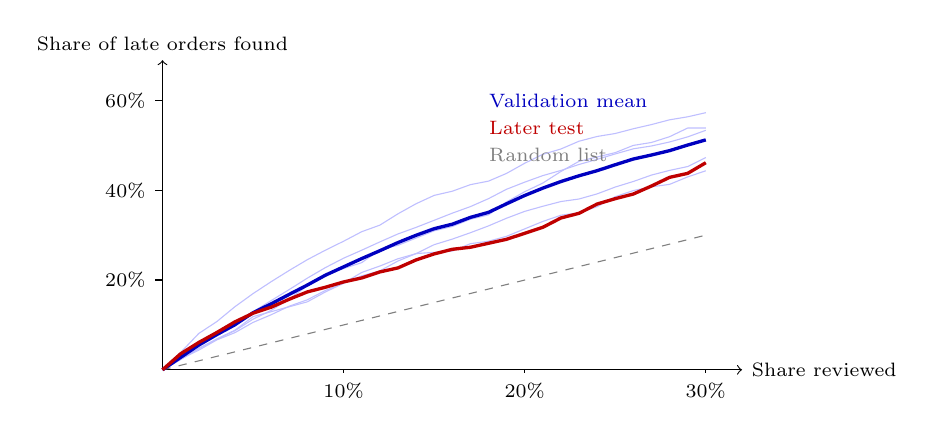
\begin{tikzpicture}[x=23cm,y=5.7cm]
\draw[->] (0,0)--(.32,0) node[right] {\scriptsize Share reviewed};
\draw[->] (0,0)--(0,.69) node[above] {\scriptsize Share of late orders found};
\draw[dashed,gray] (0,0)--(.30,.30);
\foreach \x/\lab in {.1/10,.2/20,.3/30} {\draw (\x,0)--(\x,-.008) node[below] {\scriptsize \lab\%};}
\foreach \y/\lab in {.2/20,.4/40,.6/60} {\draw (0,\y)--(-.004,\y) node[left] {\scriptsize \lab\%};}
\draw[blue!25,thin] (0.0000,0.0000) -- (0.0100,0.0226) -- (0.0200,0.0484) -- (0.0300,0.0677) -- (0.0400,0.0871) -- (0.0500,0.1129) -- (0.0600,0.1323) -- (0.0700,0.1581) -- (0.0800,0.1871) -- (0.0900,0.2097) -- (0.1000,0.2258) -- (0.1100,0.2387) -- (0.1200,0.2677) -- (0.1300,0.2774) -- (0.1400,0.2935) -- (0.1500,0.3097) -- (0.1600,0.3194) -- (0.1700,0.3355) -- (0.1800,0.3452) -- (0.1900,0.3742) -- (0.2000,0.3968) -- (0.2100,0.4161) -- (0.2200,0.4419) -- (0.2300,0.4645) -- (0.2400,0.4742) -- (0.2500,0.4839) -- (0.2600,0.5000) -- (0.2700,0.5065) -- (0.2800,0.5194) -- (0.2900,0.5387) -- (0.3000,0.5387);
\draw[blue!25,thin] (0.0000,0.0000) -- (0.0100,0.0238) -- (0.0200,0.0438) -- (0.0300,0.0666) -- (0.0400,0.0828) -- (0.0500,0.1056) -- (0.0600,0.1227) -- (0.0700,0.1418) -- (0.0800,0.1560) -- (0.0900,0.1770) -- (0.1000,0.1931) -- (0.1100,0.2169) -- (0.1200,0.2312) -- (0.1300,0.2474) -- (0.1400,0.2588) -- (0.1500,0.2788) -- (0.1600,0.2912) -- (0.1700,0.3054) -- (0.1800,0.3206) -- (0.1900,0.3378) -- (0.2000,0.3530) -- (0.2100,0.3644) -- (0.2200,0.3749) -- (0.2300,0.3806) -- (0.2400,0.3920) -- (0.2500,0.4072) -- (0.2600,0.4196) -- (0.2700,0.4339) -- (0.2800,0.4443) -- (0.2900,0.4529) -- (0.3000,0.4729);
\draw[blue!25,thin] (0.0000,0.0000) -- (0.0100,0.0248) -- (0.0200,0.0468) -- (0.0300,0.0689) -- (0.0400,0.0882) -- (0.0500,0.1185) -- (0.0600,0.1295) -- (0.0700,0.1405) -- (0.0800,0.1515) -- (0.0900,0.1736) -- (0.1000,0.1928) -- (0.1100,0.2094) -- (0.1200,0.2204) -- (0.1300,0.2424) -- (0.1400,0.2590) -- (0.1500,0.2617) -- (0.1600,0.2645) -- (0.1700,0.2810) -- (0.1800,0.2865) -- (0.1900,0.2975) -- (0.2000,0.3140) -- (0.2100,0.3306) -- (0.2200,0.3444) -- (0.2300,0.3499) -- (0.2400,0.3636) -- (0.2500,0.3857) -- (0.2600,0.3994) -- (0.2700,0.4077) -- (0.2800,0.4132) -- (0.2900,0.4298) -- (0.3000,0.4435);
\draw[blue!25,thin] (0.0000,0.0000) -- (0.0100,0.0385) -- (0.0200,0.0809) -- (0.0300,0.1074) -- (0.0400,0.1406) -- (0.0500,0.1698) -- (0.0600,0.1963) -- (0.0700,0.2215) -- (0.0800,0.2454) -- (0.0900,0.2666) -- (0.1000,0.2865) -- (0.1100,0.3077) -- (0.1200,0.3223) -- (0.1300,0.3475) -- (0.1400,0.3700) -- (0.1500,0.3886) -- (0.1600,0.3979) -- (0.1700,0.4125) -- (0.1800,0.4204) -- (0.1900,0.4377) -- (0.2000,0.4602) -- (0.2100,0.4801) -- (0.2200,0.4920) -- (0.2300,0.5093) -- (0.2400,0.5199) -- (0.2500,0.5265) -- (0.2600,0.5371) -- (0.2700,0.5464) -- (0.2800,0.5570) -- (0.2900,0.5637) -- (0.3000,0.5729);
\draw[blue!25,thin] (0.0000,0.0000) -- (0.0100,0.0286) -- (0.0200,0.0552) -- (0.0300,0.0812) -- (0.0400,0.1028) -- (0.0500,0.1294) -- (0.0600,0.1542) -- (0.0700,0.1789) -- (0.0800,0.2043) -- (0.0900,0.2278) -- (0.1000,0.2487) -- (0.1100,0.2665) -- (0.1200,0.2849) -- (0.1300,0.3027) -- (0.1400,0.3173) -- (0.1500,0.3331) -- (0.1600,0.3490) -- (0.1700,0.3636) -- (0.1800,0.3813) -- (0.1900,0.4023) -- (0.2000,0.4181) -- (0.2100,0.4327) -- (0.2200,0.4442) -- (0.2300,0.4575) -- (0.2400,0.4689) -- (0.2500,0.4810) -- (0.2600,0.4924) -- (0.2700,0.4987) -- (0.2800,0.5076) -- (0.2900,0.5190) -- (0.3000,0.5336);
\draw[blue!75!black,very thick] (0.0000,0.0000) -- (0.0100,0.0276) -- (0.0200,0.0550) -- (0.0300,0.0784) -- (0.0400,0.1003) -- (0.0500,0.1272) -- (0.0600,0.1470) -- (0.0700,0.1681) -- (0.0800,0.1889) -- (0.0900,0.2109) -- (0.1000,0.2294) -- (0.1100,0.2478) -- (0.1200,0.2653) -- (0.1300,0.2835) -- (0.1400,0.2997) -- (0.1500,0.3144) -- (0.1600,0.3244) -- (0.1700,0.3396) -- (0.1800,0.3508) -- (0.1900,0.3699) -- (0.2000,0.3884) -- (0.2100,0.4048) -- (0.2200,0.4195) -- (0.2300,0.4323) -- (0.2400,0.4437) -- (0.2500,0.4569) -- (0.2600,0.4697) -- (0.2700,0.4786) -- (0.2800,0.4883) -- (0.2900,0.5008) -- (0.3000,0.5123);
\draw[red!75!black,very thick] (0.0000,0.0000) -- (0.0100,0.0356) -- (0.0200,0.0608) -- (0.0300,0.0831) -- (0.0400,0.1068) -- (0.0500,0.1261) -- (0.0600,0.1395) -- (0.0700,0.1573) -- (0.0800,0.1736) -- (0.0900,0.1840) -- (0.1000,0.1958) -- (0.1100,0.2047) -- (0.1200,0.2181) -- (0.1300,0.2270) -- (0.1400,0.2448) -- (0.1500,0.2582) -- (0.1600,0.2685) -- (0.1700,0.2730) -- (0.1800,0.2819) -- (0.1900,0.2908) -- (0.2000,0.3042) -- (0.2100,0.3175) -- (0.2200,0.3383) -- (0.2300,0.3487) -- (0.2400,0.3694) -- (0.2500,0.3813) -- (0.2600,0.3917) -- (0.2700,0.4095) -- (0.2800,0.4288) -- (0.2900,0.4377) -- (0.3000,0.4614);
\node[anchor=west,blue!75!black] at (.175,.60) {\scriptsize Validation mean};
\node[anchor=west,red!75!black] at (.175,.54) {\scriptsize Later test};
\node[anchor=west,gray] at (.175,.48) {\scriptsize Random list};
\end{tikzpicture}
% END GENERATED GAINS FIGURE
\caption{Cumulative gains: a shorter risk-ranked list finds more late orders than a random list. Test-period operating points are exploratory.}
\label{fig:gains}
\end{figure}

\begin{table}[h]
\centering\small
\caption{Precision and recall at review capacities of 1--20\%. Validation values are means of five within-window results. Test precision includes 95\% order-bootstrap intervals; every test top-$k$ value is post hoc.}
\label{tab:topk}
\begin{tabular}{@{}rrrrr@{}}
\toprule
Share reviewed & Validation precision & Validation recall & Test precision (95\% interval) & Test recall \\
\midrule
1\% & 29.9\% & 2.8\% & 12.4\% (7.7--17.0\%) & 3.6\% \\
5\% & 27.3\% & 12.7\% & 8.8\% (7.0--10.4\%) & 12.6\% \\
10\% & 25.0\% & 22.9\% & 6.8\% (5.8--8.0\%) & 19.6\% \\
20\% & 21.2\% & 38.8\% & 5.3\% (4.6--6.0\%) & 30.4\% \\
\bottomrule
\end{tabular}
\end{table}

At 10\% capacity, the exploratory test list contains 1,937 orders and 132 late deliveries. Its 6.8\% precision is about twice the test late rate, but it still misses four in five late deliveries. If a review prevents a fraction $e$ of the late deliveries it identifies, the direct review cost would need to be below $0.068e$ times the cost of a late delivery just to break even against no review. We do not know $e$ or the costs from these data.

\section*{Why the fixed alert rule did not transfer}
The preselected yes/no rule used the probability cutoff 0.0788, chosen to maximise Matthews correlation coefficient (MCC) on pooled validation predictions. This pools five models fitted at different times and late rates. The same numeric cutoff flagged 9.5\% of validation orders but 42.9\% of test orders. The final refit also assigned a higher mean risk in the test (9.82\%) than the observed late rate (3.48\%); validation predictions had the opposite pattern in every window (Table~\ref{tab:periods}). Figure~\ref{fig:calibration} shows the same mismatch within five equal-count score groups per period. The curves show that predicted probabilities are not well calibrated across periods. They do not establish whether changing order mix, prevalence, model refitting or another factor caused the shift.

\begin{figure}[h]
\centering
% BEGIN GENERATED CALIBRATION FIGURE
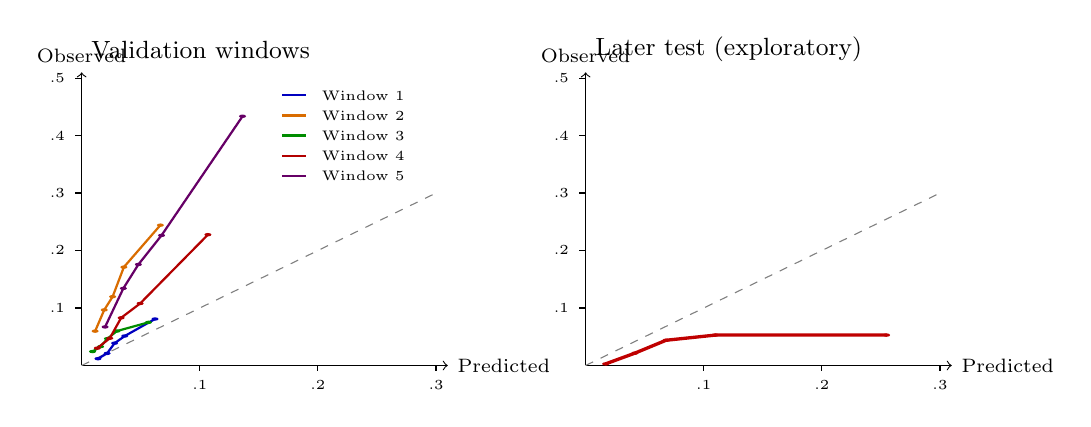
\begin{tikzpicture}[x=15cm,y=7.3cm]
\begin{scope}[xshift=0cm]
\draw[->] (0,0)--(.31,0) node[right] {\scriptsize Predicted};
\draw[->] (0,0)--(0,.51) node[above] {\scriptsize Observed};
\draw[dashed,gray] (0,0)--(.30,.30);
\foreach \v in {.1,.2,.3} {\draw (\v,0)--(\v,-.009) node[below] {\tiny \v};}
\foreach \v in {.1,.2,.3,.4,.5} {\draw (0,\v)--(-.006,\v) node[left] {\tiny \v};}
\node[anchor=west] at (0,.55) {\small Validation windows};
\draw[blue!75!black,thick] (0.0138,0.0118) -- (0.0215,0.0211) -- (0.0279,0.0388) -- (0.0365,0.0513) -- (0.0621,0.0809);
\fill[blue!75!black] (0.0138,0.0118) circle[radius=.003];
\fill[blue!75!black] (0.0215,0.0211) circle[radius=.003];
\fill[blue!75!black] (0.0279,0.0388) circle[radius=.003];
\fill[blue!75!black] (0.0365,0.0513) circle[radius=.003];
\fill[blue!75!black] (0.0621,0.0809) circle[radius=.003];
\draw[orange!85!black,thick] (0.0114,0.0598) -- (0.0191,0.0967) -- (0.0262,0.1197) -- (0.0357,0.1711) -- (0.0666,0.2441);
\fill[orange!85!black] (0.0114,0.0598) circle[radius=.003];
\fill[orange!85!black] (0.0191,0.0967) circle[radius=.003];
\fill[orange!85!black] (0.0262,0.1197) circle[radius=.003];
\fill[orange!85!black] (0.0357,0.1711) circle[radius=.003];
\fill[orange!85!black] (0.0666,0.2441) circle[radius=.003];
\draw[green!55!black,thick] (0.0092,0.0243) -- (0.0160,0.0329) -- (0.0218,0.0467) -- (0.0298,0.0599) -- (0.0565,0.0750);
\fill[green!55!black] (0.0092,0.0243) circle[radius=.003];
\fill[green!55!black] (0.0160,0.0329) circle[radius=.003];
\fill[green!55!black] (0.0218,0.0467) circle[radius=.003];
\fill[green!55!black] (0.0298,0.0599) circle[radius=.003];
\fill[green!55!black] (0.0565,0.0750) circle[radius=.003];
\draw[red!70!black,thick] (0.0132,0.0302) -- (0.0238,0.0474) -- (0.0334,0.0829) -- (0.0495,0.1079) -- (0.1069,0.2276);
\fill[red!70!black] (0.0132,0.0302) circle[radius=.003];
\fill[red!70!black] (0.0238,0.0474) circle[radius=.003];
\fill[red!70!black] (0.0334,0.0829) circle[radius=.003];
\fill[red!70!black] (0.0495,0.1079) circle[radius=.003];
\fill[red!70!black] (0.1069,0.2276) circle[radius=.003];
\draw[violet!80!black,thick] (0.0198,0.0671) -- (0.0353,0.1342) -- (0.0480,0.1757) -- (0.0676,0.2263) -- (0.1362,0.4336);
\fill[violet!80!black] (0.0198,0.0671) circle[radius=.003];
\fill[violet!80!black] (0.0353,0.1342) circle[radius=.003];
\fill[violet!80!black] (0.0480,0.1757) circle[radius=.003];
\fill[violet!80!black] (0.0676,0.2263) circle[radius=.003];
\fill[violet!80!black] (0.1362,0.4336) circle[radius=.003];
\draw[blue!75!black,thick] (0.1700,0.4700) -- (0.1900,0.4700);
\node[anchor=west] at (0.1950,0.4700) {\tiny Window 1};
\draw[orange!85!black,thick] (0.1700,0.4350) -- (0.1900,0.4350);
\node[anchor=west] at (0.1950,0.4350) {\tiny Window 2};
\draw[green!55!black,thick] (0.1700,0.4000) -- (0.1900,0.4000);
\node[anchor=west] at (0.1950,0.4000) {\tiny Window 3};
\draw[red!70!black,thick] (0.1700,0.3650) -- (0.1900,0.3650);
\node[anchor=west] at (0.1950,0.3650) {\tiny Window 4};
\draw[violet!80!black,thick] (0.1700,0.3300) -- (0.1900,0.3300);
\node[anchor=west] at (0.1950,0.3300) {\tiny Window 5};
\end{scope}
\begin{scope}[xshift=6.4cm]
\draw[->] (0,0)--(.31,0) node[right] {\scriptsize Predicted};
\draw[->] (0,0)--(0,.51) node[above] {\scriptsize Observed};
\draw[dashed,gray] (0,0)--(.30,.30);
\foreach \v in {.1,.2,.3} {\draw (\v,0)--(\v,-.009) node[below] {\tiny \v};}
\foreach \v in {.1,.2,.3,.4,.5} {\draw (0,\v)--(-.006,\v) node[left] {\tiny \v};}
\node[anchor=west] at (0,.55) {\small Later test (exploratory)};
\draw[red!75!black,very thick] (0.0169,0.0028) -- (0.0416,0.0214) -- (0.0681,0.0439) -- (0.1098,0.0529) -- (0.2548,0.0529);
\fill[red!75!black] (0.0169,0.0028) circle[radius=.003];
\fill[red!75!black] (0.0416,0.0214) circle[radius=.003];
\fill[red!75!black] (0.0681,0.0439) circle[radius=.003];
\fill[red!75!black] (0.1098,0.0529) circle[radius=.003];
\fill[red!75!black] (0.2548,0.0529) circle[radius=.003];
\end{scope}
\end{tikzpicture}
% END GENERATED CALIBRATION FIGURE
\caption{Predicted risk versus observed late rate in five equal-count score groups per period. The dashed line means exact agreement. Test calibration is a post-hoc diagnostic.}
\label{fig:calibration}
\end{figure}

\begin{table}[h]
\centering\small
\caption{Secondary yes/no alert results at the unchanged validation-selected cutoff of 0.0788. Validation alert metrics use the same predictions that selected the cutoff and are optimistic.}
\label{tab:heldout}
\begin{tabular}{@{}lrr@{}}
\toprule
Measure & Pooled validation & Later test \\
\midrule
Orders flagged & 3,600 (9.5\%) & 8,316 (42.9\%) \\
True / false alerts & 1,145 / 2,455 & 434 / 7,882 \\
Late orders missed & 2,909 & 240 \\
Precision / recall & 31.8\% / 28.2\% & 5.2\% / 64.4\% \\
F1 / MCC & 0.299 / 0.222 & 0.097 / 0.082 \\
\bottomrule
\end{tabular}
\end{table}

This cutoff is impractical for a small team and should not trigger expensive intervention or a message telling a customer that a particular order will be late. Choosing another absolute cutoff, calibrating on test labels, or switching to a test-selected quantile rule would use the held-out period for tuning. We retain the original result and treat the top-$k$ view as a possible policy to validate prospectively.

\section*{Exploratory period and missing-outcome checks}
The pooled test score hides large within-period differences (Table~\ref{tab:months}). June ranking was stronger than August ranking; August ROC-AUC was only 0.522, with an order-bootstrap interval spanning 0.5. The late rate also rose from 1.2\% in June to 6.2\% in August. These monthly results and intervals are post-hoc diagnostics, not new independent tests. In particular, the pooled ROC-AUC of 0.668 does not imply stable performance in every month.

\begin{table}[h]
\centering\scriptsize
\caption{Post-hoc monthly test results. Parentheses give 95\% order-bootstrap intervals from 1,000 resamples per month. Precision is for each month's top 10\%.}
\label{tab:months}
\begin{tabular}{@{}lrrrrr@{}}
\toprule
Purchase month & Late / orders & PR-AUC (interval) & PR-AUC / rate & ROC-AUC (interval) & Top-10\% precision (interval) \\
\midrule
Jun 2018 & 71 / 6,096 & 0.060 (0.035--0.113) & 5.14 & 0.761 (0.706--0.814) & 3.8\% (2.5--5.6\%) \\
Jul 2018 & 208 / 6,156 & 0.063 (0.050--0.089) & 1.88 & 0.634 (0.595--0.673) & 7.8\% (5.7--9.9\%) \\
Aug 2018 & 393 / 6,351 & 0.074 (0.062--0.096) & 1.20 & 0.522 (0.496--0.549) & 7.4\% (5.3--9.4\%) \\
\bottomrule
\end{tabular}
\end{table}

There are also 193 purchases from 26 May to 31 August still marked as in progress with no observed delivery: 3 in May, 46 in June, 74 in July and 70 in August. Their eventual delivery outcomes are unknown, so they cannot be assigned a late-delivery label or included in the delivered-only model evaluation. This missing-outcome pattern may affect the observed late rate, especially for recent purchases, but does not establish the cause or size of the PR-AUC drop. Cancelled and unavailable orders are outside this delivered-order question.

Higher scores in public Olist notebooks are not directly comparable when they use a random split, a different late definition, or information recorded after checkout. In our own primary training period, a shuffled, stratified check gave logistic mean PR-AUC 0.303, compared with 0.200 for chronological validation. Mixing periods makes this particular task easier; it does not measure how the checkout model works on future purchases.

\section*{Business conclusion}
The model shows a modest ability to rank delivered orders by late-delivery risk, but the fixed yes/no alert rule did not transfer across periods and checkout information does not support dependable individual alerts. A low-cost watchlist could be piloted only with a clear action, review capacity and measured costs. Later signals, especially slow carrier handover, might support a second prediction and would need their own future-period evaluation. This retrospective delivered-only analysis does not show that reviewing an order prevents a delay.

% Insert the team's regression analysis and joint conclusion before the appendix.
\clearpage
\appendix
\section{Classification candidate grid}
\label{app:grid}
All rows use the final checkout feature set and the same five chronological validation windows. PR-AUC is the mean of the five window scores. The constant-risk baseline is included for reference; $C$ is inverse regularisation strength. The unweighted models were trained at the natural late-order rate.

\begin{center}\small
\begin{tabular}{@{}p{0.28\linewidth}p{0.47\linewidth}r@{}}
\toprule
Candidate & Settings & Mean PR-AUC \\
\midrule
Prior baseline & Training-fold late rate for every order & 0.1067 \\
Logistic baseline & $C=1$, no class weighting & 0.1913 \\
Logistic $C=0.1$ & Stronger regularisation, no class weighting & 0.2003 \\
Logistic $C=10$ & Weaker regularisation, no class weighting & 0.1884 \\
Logistic balanced & $C=1$, balanced class weights & 0.1872 \\
Single tree baseline & No depth or leaf-size limit & 0.1107 \\
Single tree, depth 6 & Maximum depth 6; at least 50 orders per leaf & 0.1495 \\
Single tree, depth 12 & Maximum depth 12; at least 20 per leaf & 0.1414 \\
Single tree, balanced & Depth 12; leaf 20; balanced weights & 0.1392 \\
Forest baseline & 200 trees; unrestricted depth; leaf 1 & 0.1808 \\
Forest, depth 12 & 200 trees; maximum depth 12; leaf 20 & 0.1999 \\
Forest, leaf 20 & 200 trees; unrestricted depth; leaf 20 & 0.1985 \\
Forest, balanced & 200 trees; unrestricted depth; leaf 20; balanced subsample weights & 0.1967 \\
\bottomrule
\end{tabular}
\end{center}

After the primary model and test result were reported, an exploratory XGBoost check on the same training-period validation windows gave mean PR-AUC 0.2046 for a shallow setting, versus 0.2003 for logistic regression. It won in three of five windows. Because this check followed the held-out evaluation, it did not enter the original model selection and has no new independent test score. The runnable settings and fold scores are in \texttt{experiments/phase2\_xgboost\_validation.py} and its companion JSON file.
\end{document}
